\section{Painting matching}
\label{sec:painting-matching}

The elaboration of the painting matching consists of two approaches which are discussed in \ref{subsec:Keypoint matching} and \ref{subsec:Feature vector matching}. 

Realtime painting matching must have preprocessing, meaning extraction of keypoints, features and storing it into a database beforehand. The project code contains code to generate such a database. This database will be used to compare a particular painting frame with all it's contents.

\subsection{Keypoint matching}
\label{subsec:Keypoint matching}
The keypoint matching approach relies on Oriented Fast and Rotated BRIEF (ORB) feature detection. ORB is an alternative to SIFT and SURF. These algorithms are patented while ORB is not. \cite{opencvOrb}

According to reference \cite{orb_original_paper} ORB is faster than SIFT or SURF. However, in general ORB has lower correct matching results than SIFT or SURF. \cite{orb_surf_sift_evaluation} Considering the application, time is the more important factor.

Practically, two drawbacks have to be taken into account when using ORB. At first, ORB is not scale-invariant. Thus the detected images should be scaled back to the original size of the image painting stored in the database. For this application, all images are scaled with a fixed width of 800. The second drawback is the influence due to shearing. Matching sheared images implies lower matching scores. \cite{orb_surf_sift_evaluation} This particular drawback is countered by the rectification step.

Another practical issue due to blurry painting detection was established. Blurry images can cause lots of wrong matching results. This issue is mainly prevented by the wavelet filters as described in \ref{subsec:blur-detection}.

In addition to the choice for ORB, the correct matching algorithm had to be determined. OpenCV provides two types of matching algorithms: Fast Library for Approximate Nearest Neighbors (FLANN)-based and brute-force (BF)-based. FLANN matching works faster than BF matcher in case of a large dataset (high amount of key points). Considering the acceptable results (discussed below) based on BF matching the FLANN version wasn't used. \cite{opencv_matching}


%https://docs.opencv.org/4.x/d3/da1/classcv_1_1BFMatcher.html


%https://ieeexplore.ieee.org/abstract/document/6126544?casa_token=CE2fQN6_JwIAAAAA:Inx7X3B3EFlZwekm56UJ4MjTaydpL0emtOb9sEuQmkPS037HKoHzsNvr_KFYqMiwOKrJCe3HgJA

%https://www.inderscienceonline.com/doi/abs/10.1504/IJFE.2021.118910

ORB relies on one important variable, the number of key points (features called in OpenCV). Changing this variable should result in a difference in the matching score, distances between matches, and execution time.

Table \ref{tab:keypoint_feature_variation} shows us the positive and negative matches for each amount of keypoints. In total 437 images were evaluated, they were retrieved from the given dataset. As can be seen in table \ref{tab:keypoint_feature_variation} only a slightly better score is reached when increasing the number of keypoints above 100.  Based on this result the final solution is restricted to 100 keypoints. Only the 20 largest distances (keypoint distance) for a particular image are summed to obtain a distance value for each image in the database.
%true/false matching


\renewcommand{\arraystretch}{1.2}
\begin{table}[htbp]
    \caption{Keypoint/feature variation correctness results}
    \centering
    \begin{center}
        \begin{tabular}{ |c|c|c|c|  }
        %  \hline
        %  \multicolumn{4}{|c|}{Keypoint/feature variation correctness results.} \\
         \hline
         No. keypoints& Positive matches &Negative matches&Mean score (\%)\\
         \hline \hline
         50  & 402 & 35 & 91.99\\
         \hline
         100 & 423 & 14 & 96.80\\
         \hline
         200 & 424 & 13 & 97.03\\
         \hline
         300 & 425 & 12 & 97.24\\
         \hline
        \end{tabular}
    \end{center}
    \label{tab:keypoint_feature_variation}
\end{table}

Distance distributions for matches are also interesting to determine useful information about the matching. Figure \ref{fig:bxplt_distances_keypoints} shows the distance distribution for the correct and incorrect matches. The correct distance matching distribution shows many outliers in the case of the matcher with only 50 keypoints. The amount of outliers decreases as the number of keypoints/features increases. The median for each scenario also decreases as the amount of features increases. It implies fewer high matching distances. The same findings are reflected in the case of incorrect matches. In addition, it can be determined that the distance range for the correct and incorrect matches shrinks as the number of keypoints grows. Table \ref{tab:keypoint_distance_mean} confirms this fact based on the means. 


% \begin{figure*}[htbp]
%     % 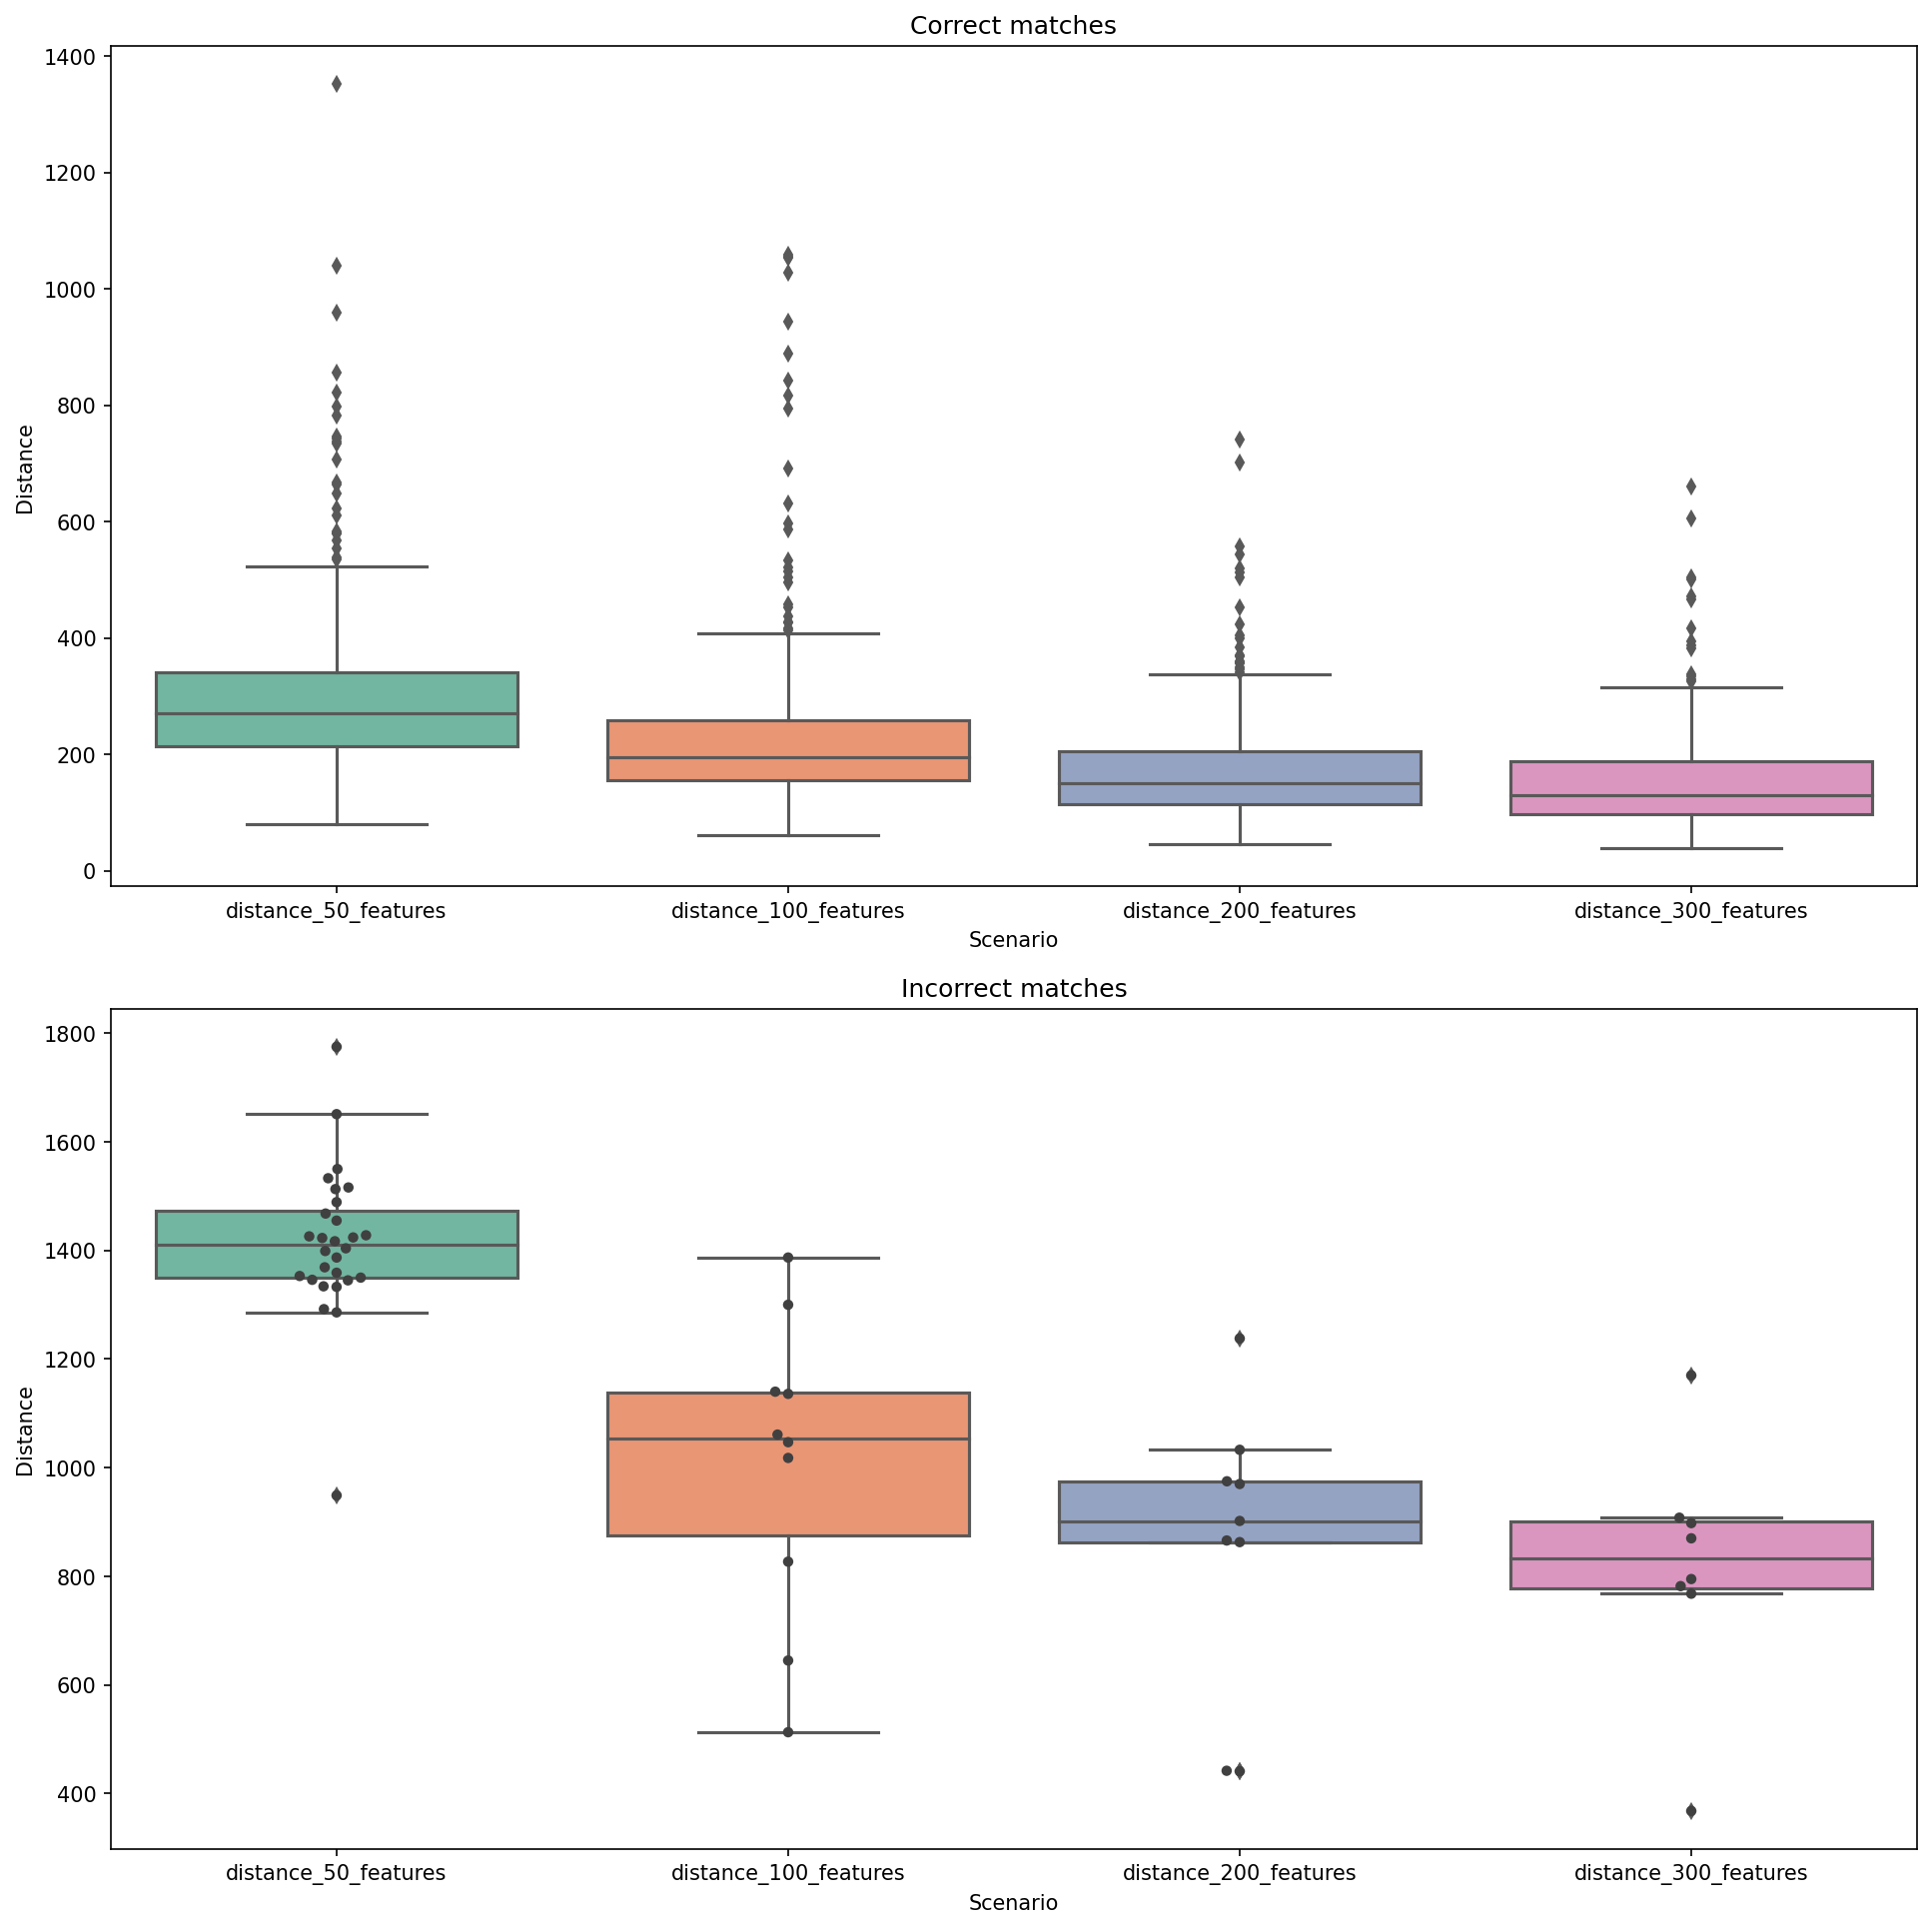
\includegraphics[width=\textwidth]{images/bxplt_distance_keypoints.png}
%     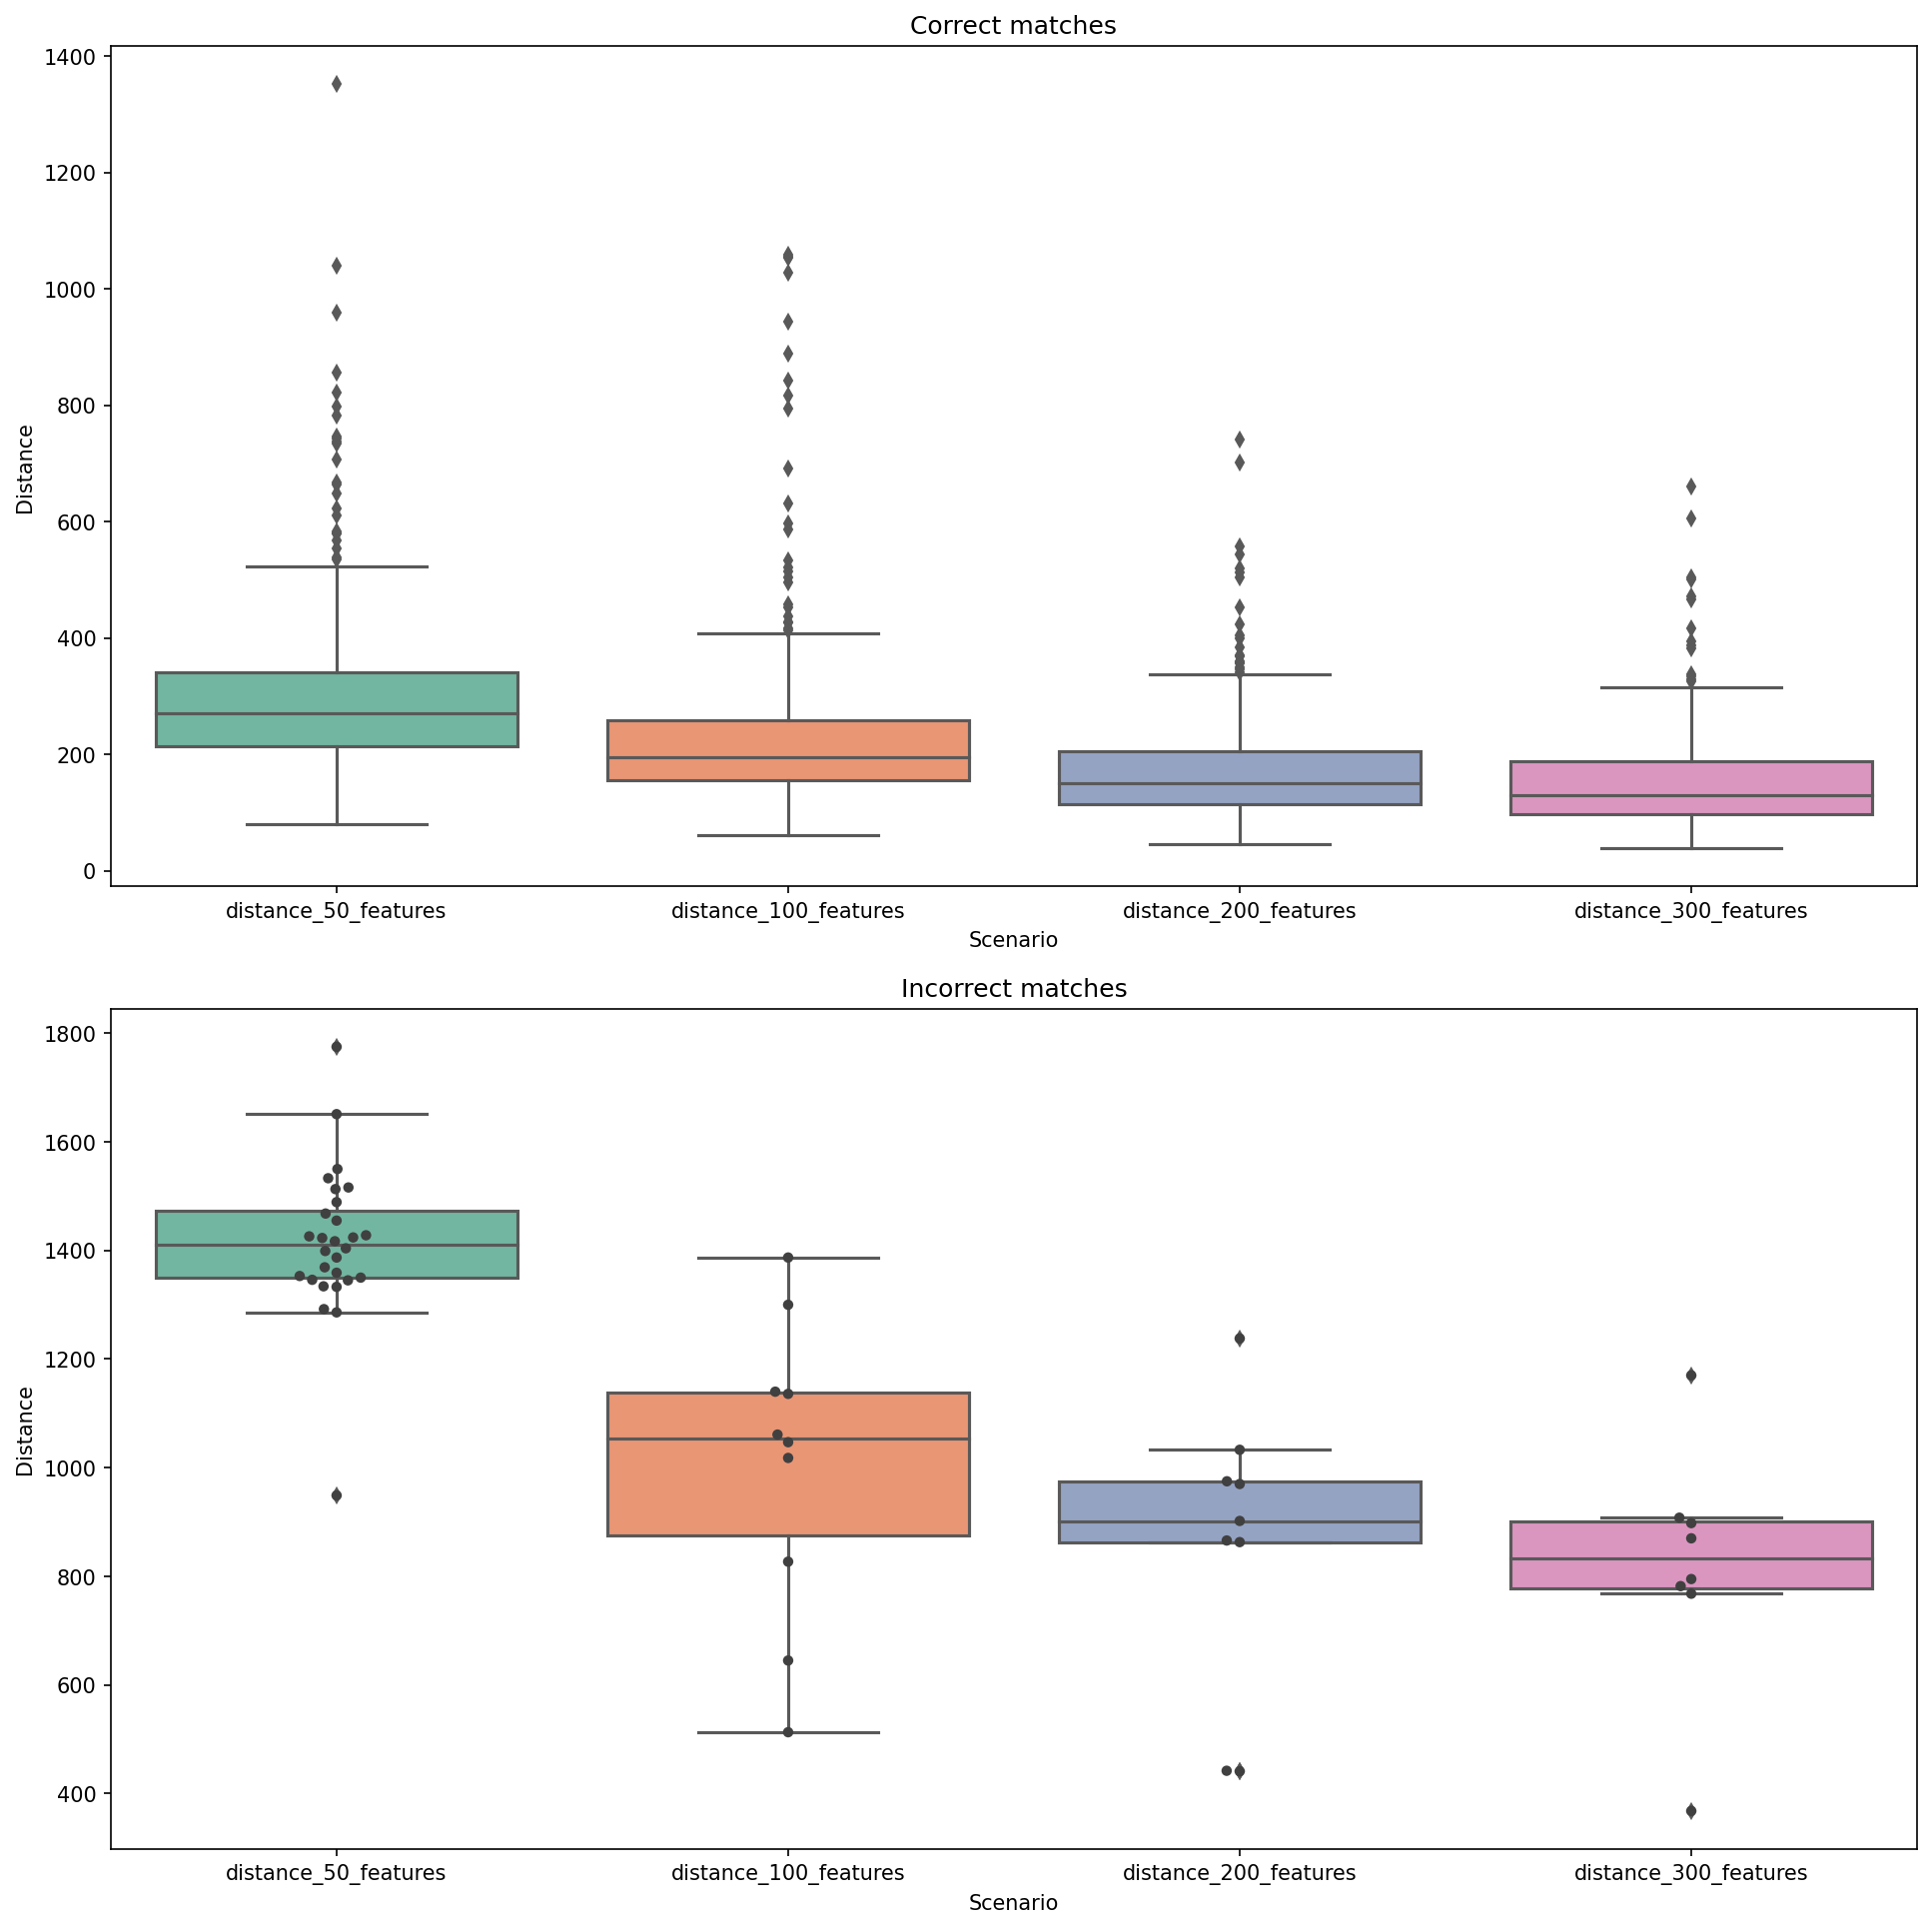
\includegraphics[width=1.6\columnwidth]{images/bxplt_distance_keypoints.png}
%     \centering
%     \caption{Distance distribution correct matches}
%     \label{fig:bxplt_distances_keypoints}
% \end{figure*}

\begin{figure}[htbp]
    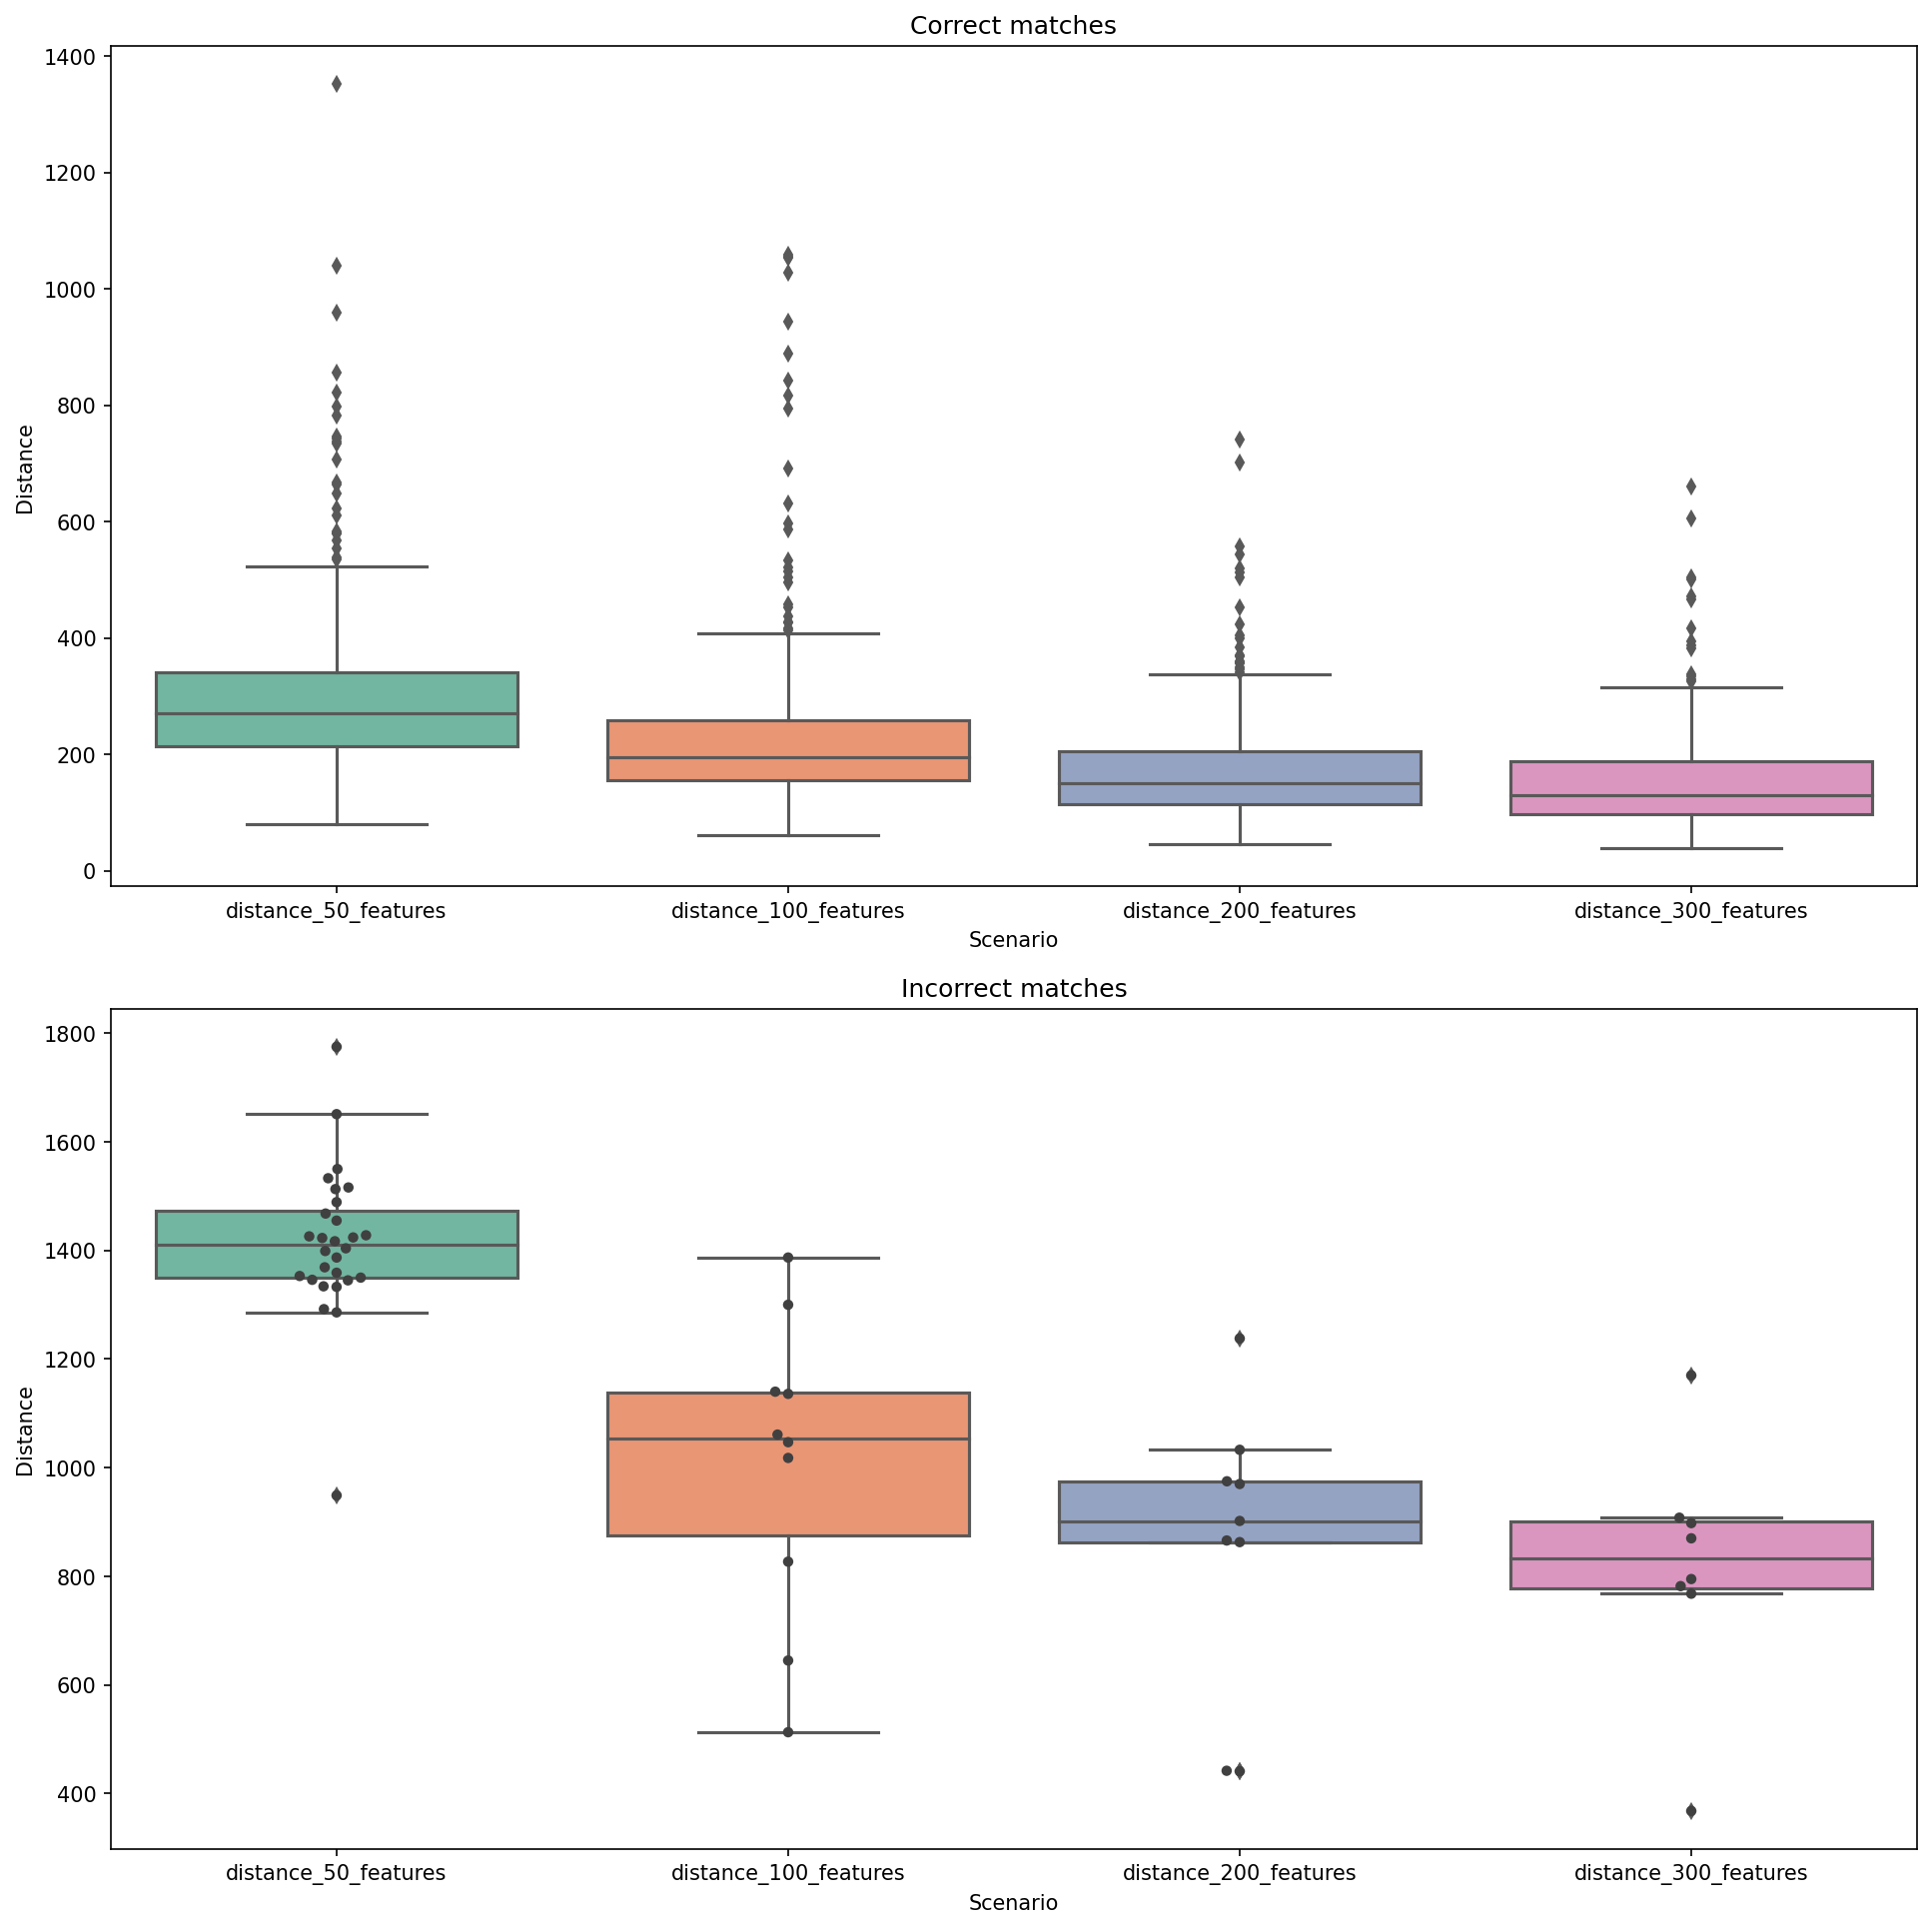
\includegraphics[width=1.0\columnwidth]{images/bxplt_distance_keypoints.png}
    \centering
    \caption{Distance distribution matches (variation of keypoints)}
    \label{fig:bxplt_distances_keypoints}
\end{figure}



\renewcommand{\arraystretch}{1.2}
\begin{table}[htbp]
    \caption{Distance distribution average values}
    \centering
    \begin{center}
        \begin{tabular}{ |c|c|c|c|  }
        %  \hline
        %  \multicolumn{4}{|c|}{Keypoint/feature variation correctness results.} \\
         \hline
         No. keypoints& Mean & Mean match & Mean no match\\
         \hline \hline
         50  & 374.98 & 302.66 & 1413.36\\
         \hline
         100 & 247.87 & 229.92 & 1007.40\\
         \hline
         200 & 187.71 & 173.47 & 858.89\\
         \hline
         300 & 164.64 & 152.30 & 819.88\\
         \hline
        \end{tabular}
    \end{center}
    \label{tab:keypoint_distance_mean}
\end{table}

Most of the wrong matched images have a strong intensity deviation or contain only dark colors. (figure \ref{fig:wrong_result_dark} and figure \ref{fig:wrong_result_light}) The effect of varying intensity is reviewed in \cite{orb_surf_sift_evaluation}. SURF and SIFT are less sensitive to this and will perform better. Nonetheless, this issue does not cause much trouble when using the videos.

\begin{figure}[htbp]
    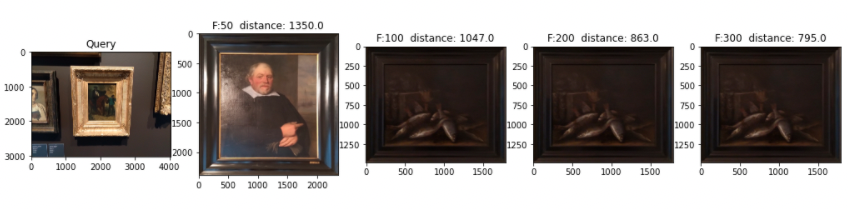
\includegraphics[width=1.0\columnwidth]{images/wrong_result cropped.png}
    \centering
    \caption{Incorrect matching results due to darkness}
    \label{fig:wrong_result_dark}
\end{figure}

\begin{figure}[htbp]
    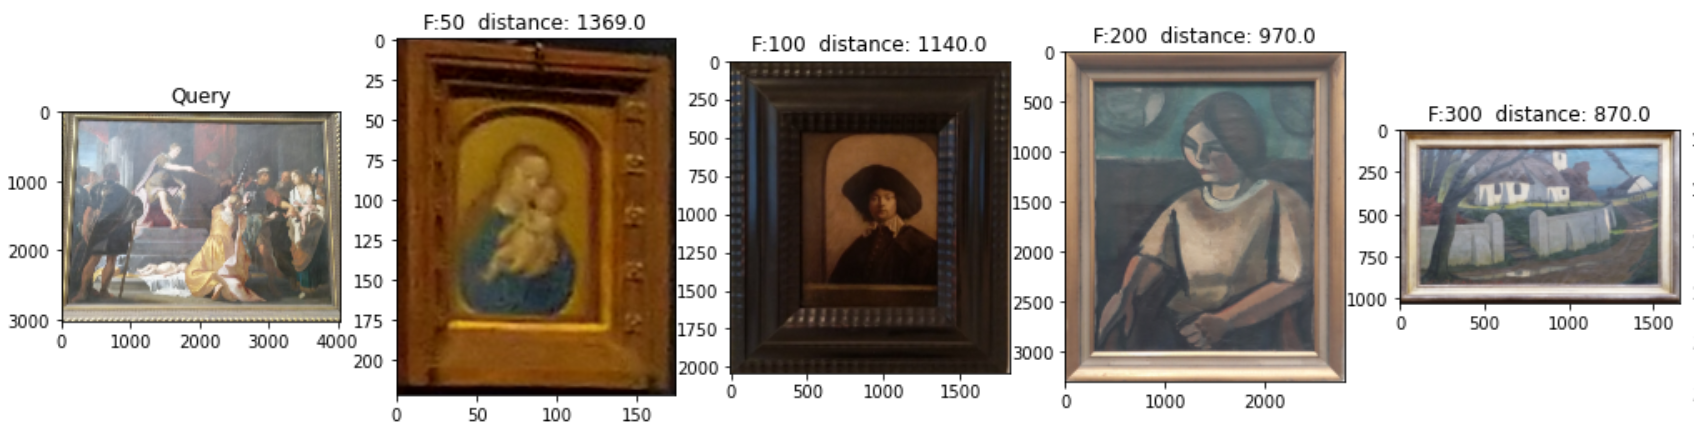
\includegraphics[width=1.0\columnwidth]{images/wrong_results_int.png}
    \centering
    \caption{Incorrect matching results due too much light}
    \label{fig:wrong_result_light}
\end{figure}

% Distance between matches

Distances between first and second matches may reflect information about the quality of a particular match. Figure \ref{fig:bxplt_difference_keypoints} confirms this assumption, the distances between the first and second matches are remarkably lower in case of incorrect matches.

% \begin{figure*}[htbp]
%     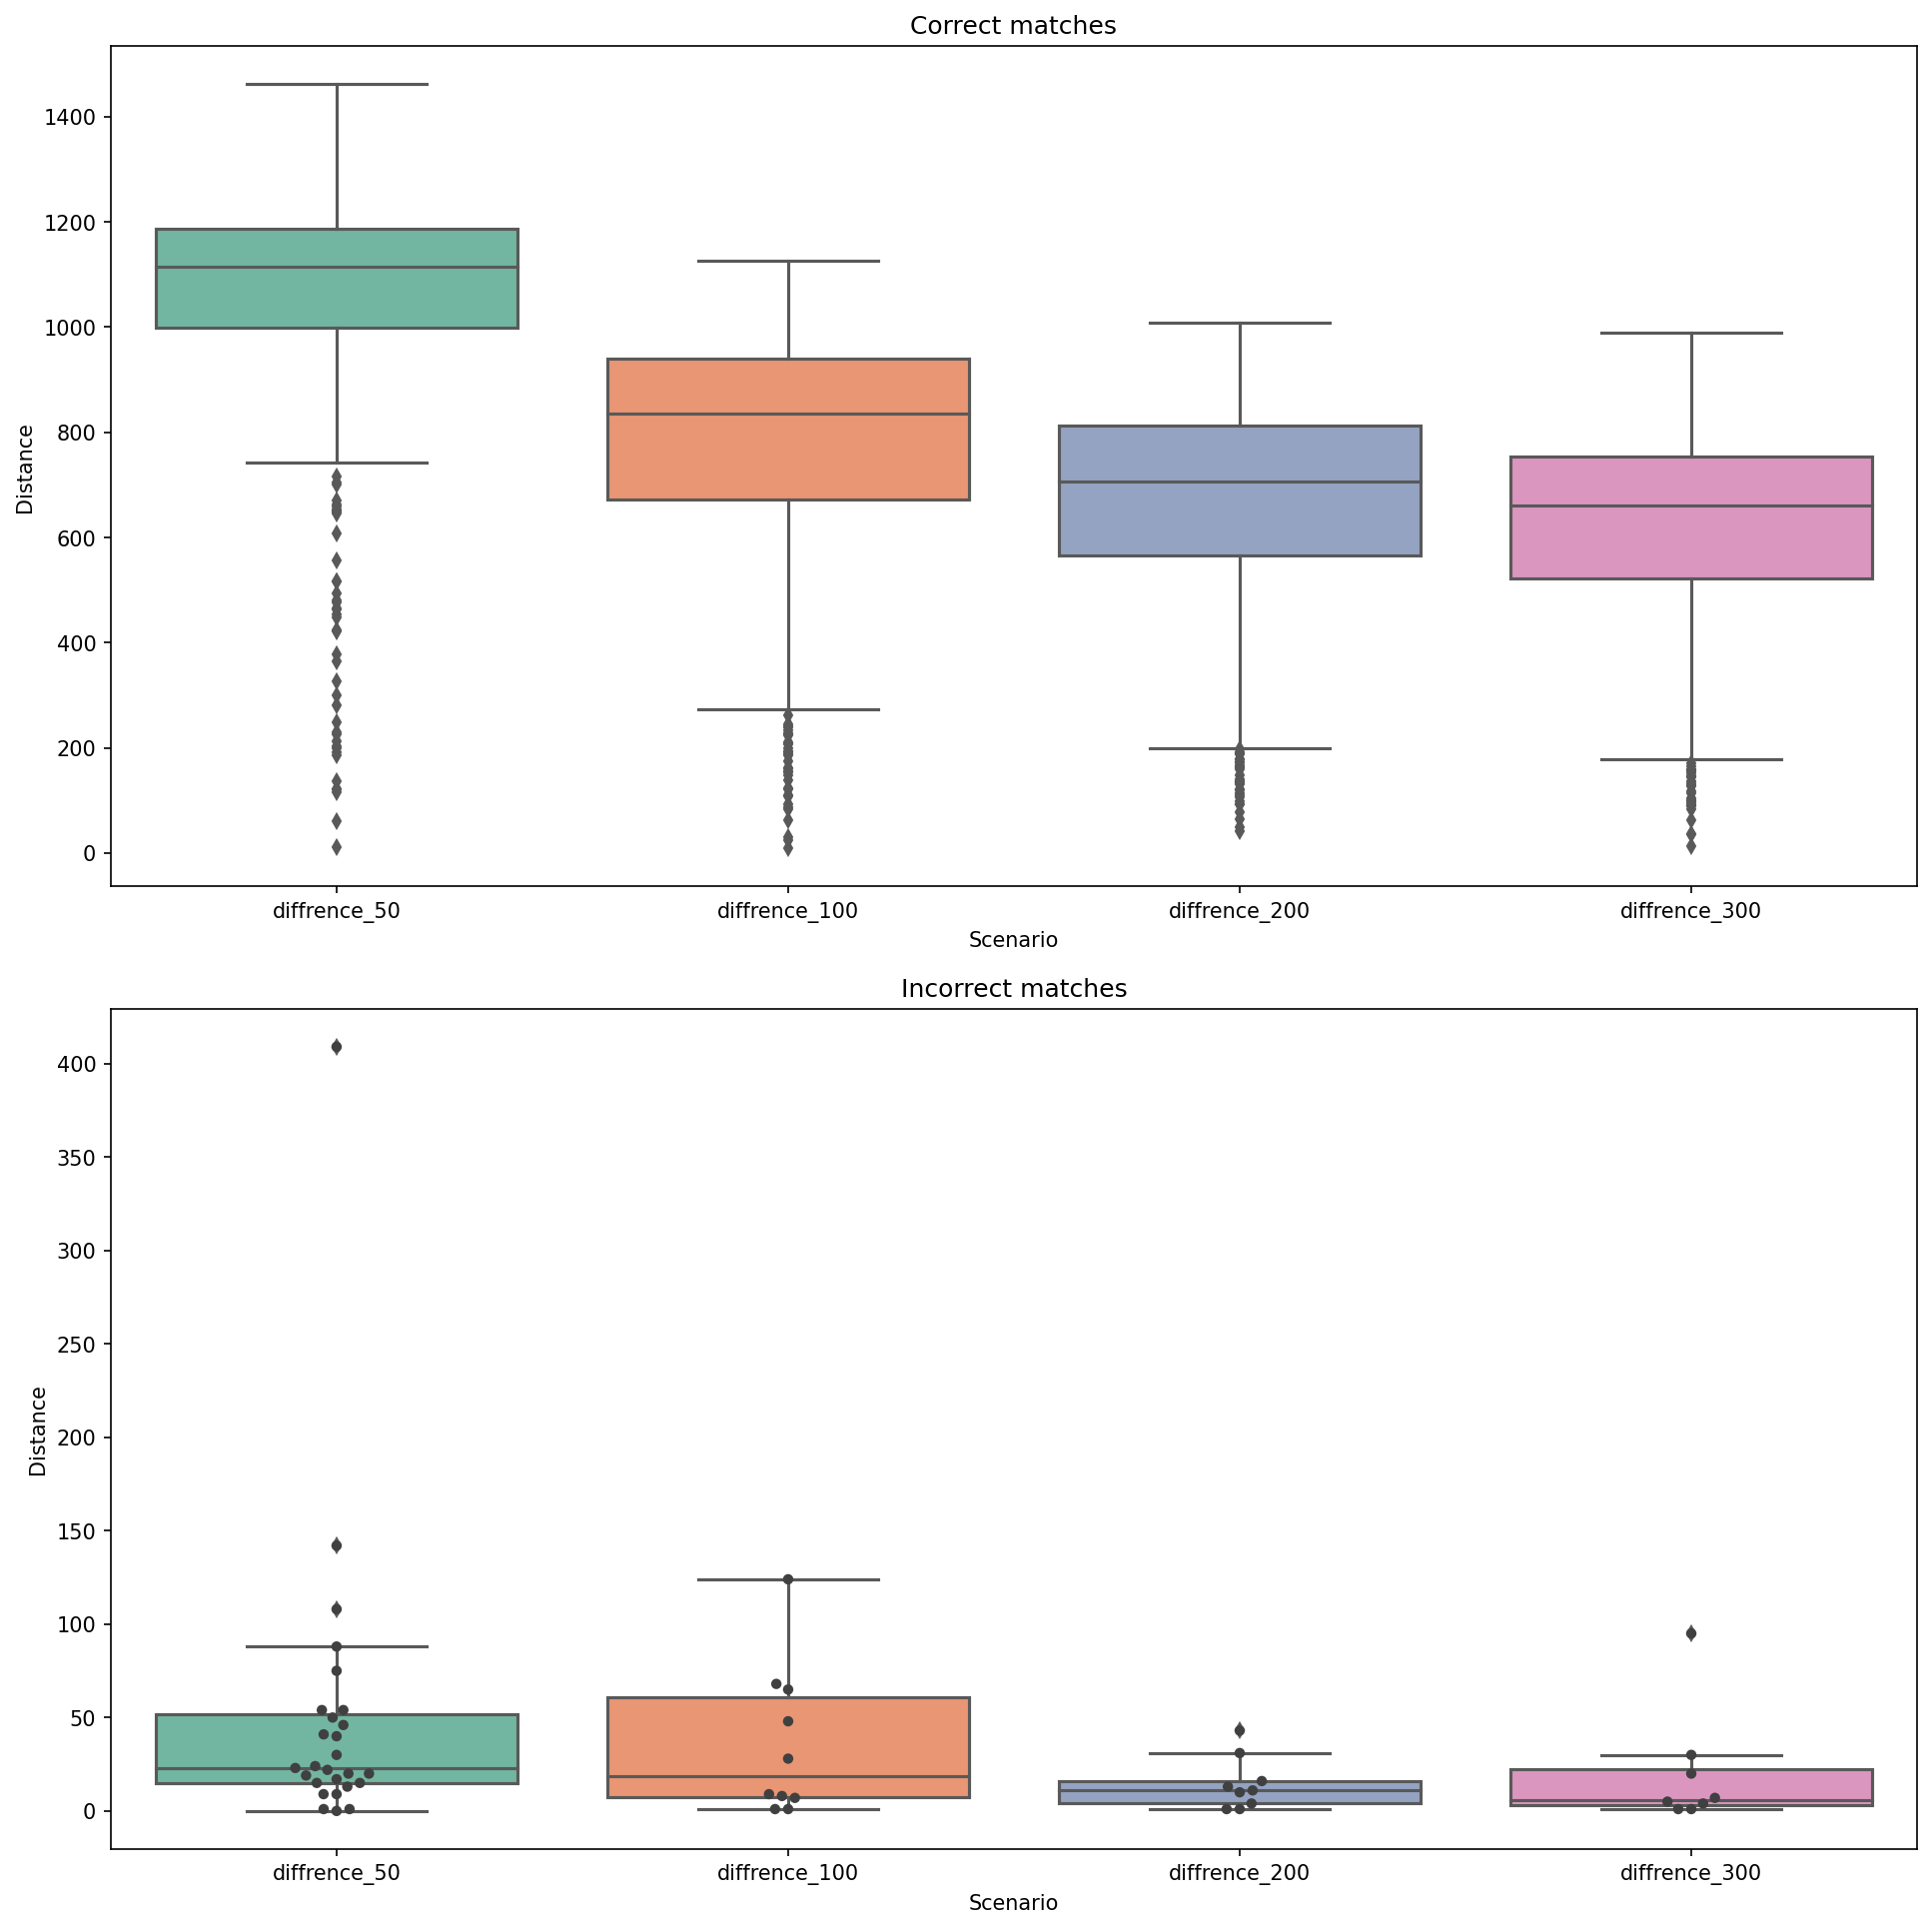
\includegraphics[width=1.6\columnwidth]{images/bxplt_difference_keypoints.png}
%     \centering
%     \caption{Difference between first and second matching result in case of correct matches}
%     \label{fig:bxplt_difference_keypoints}
% \end{figure*}

\begin{figure}[htbp]
    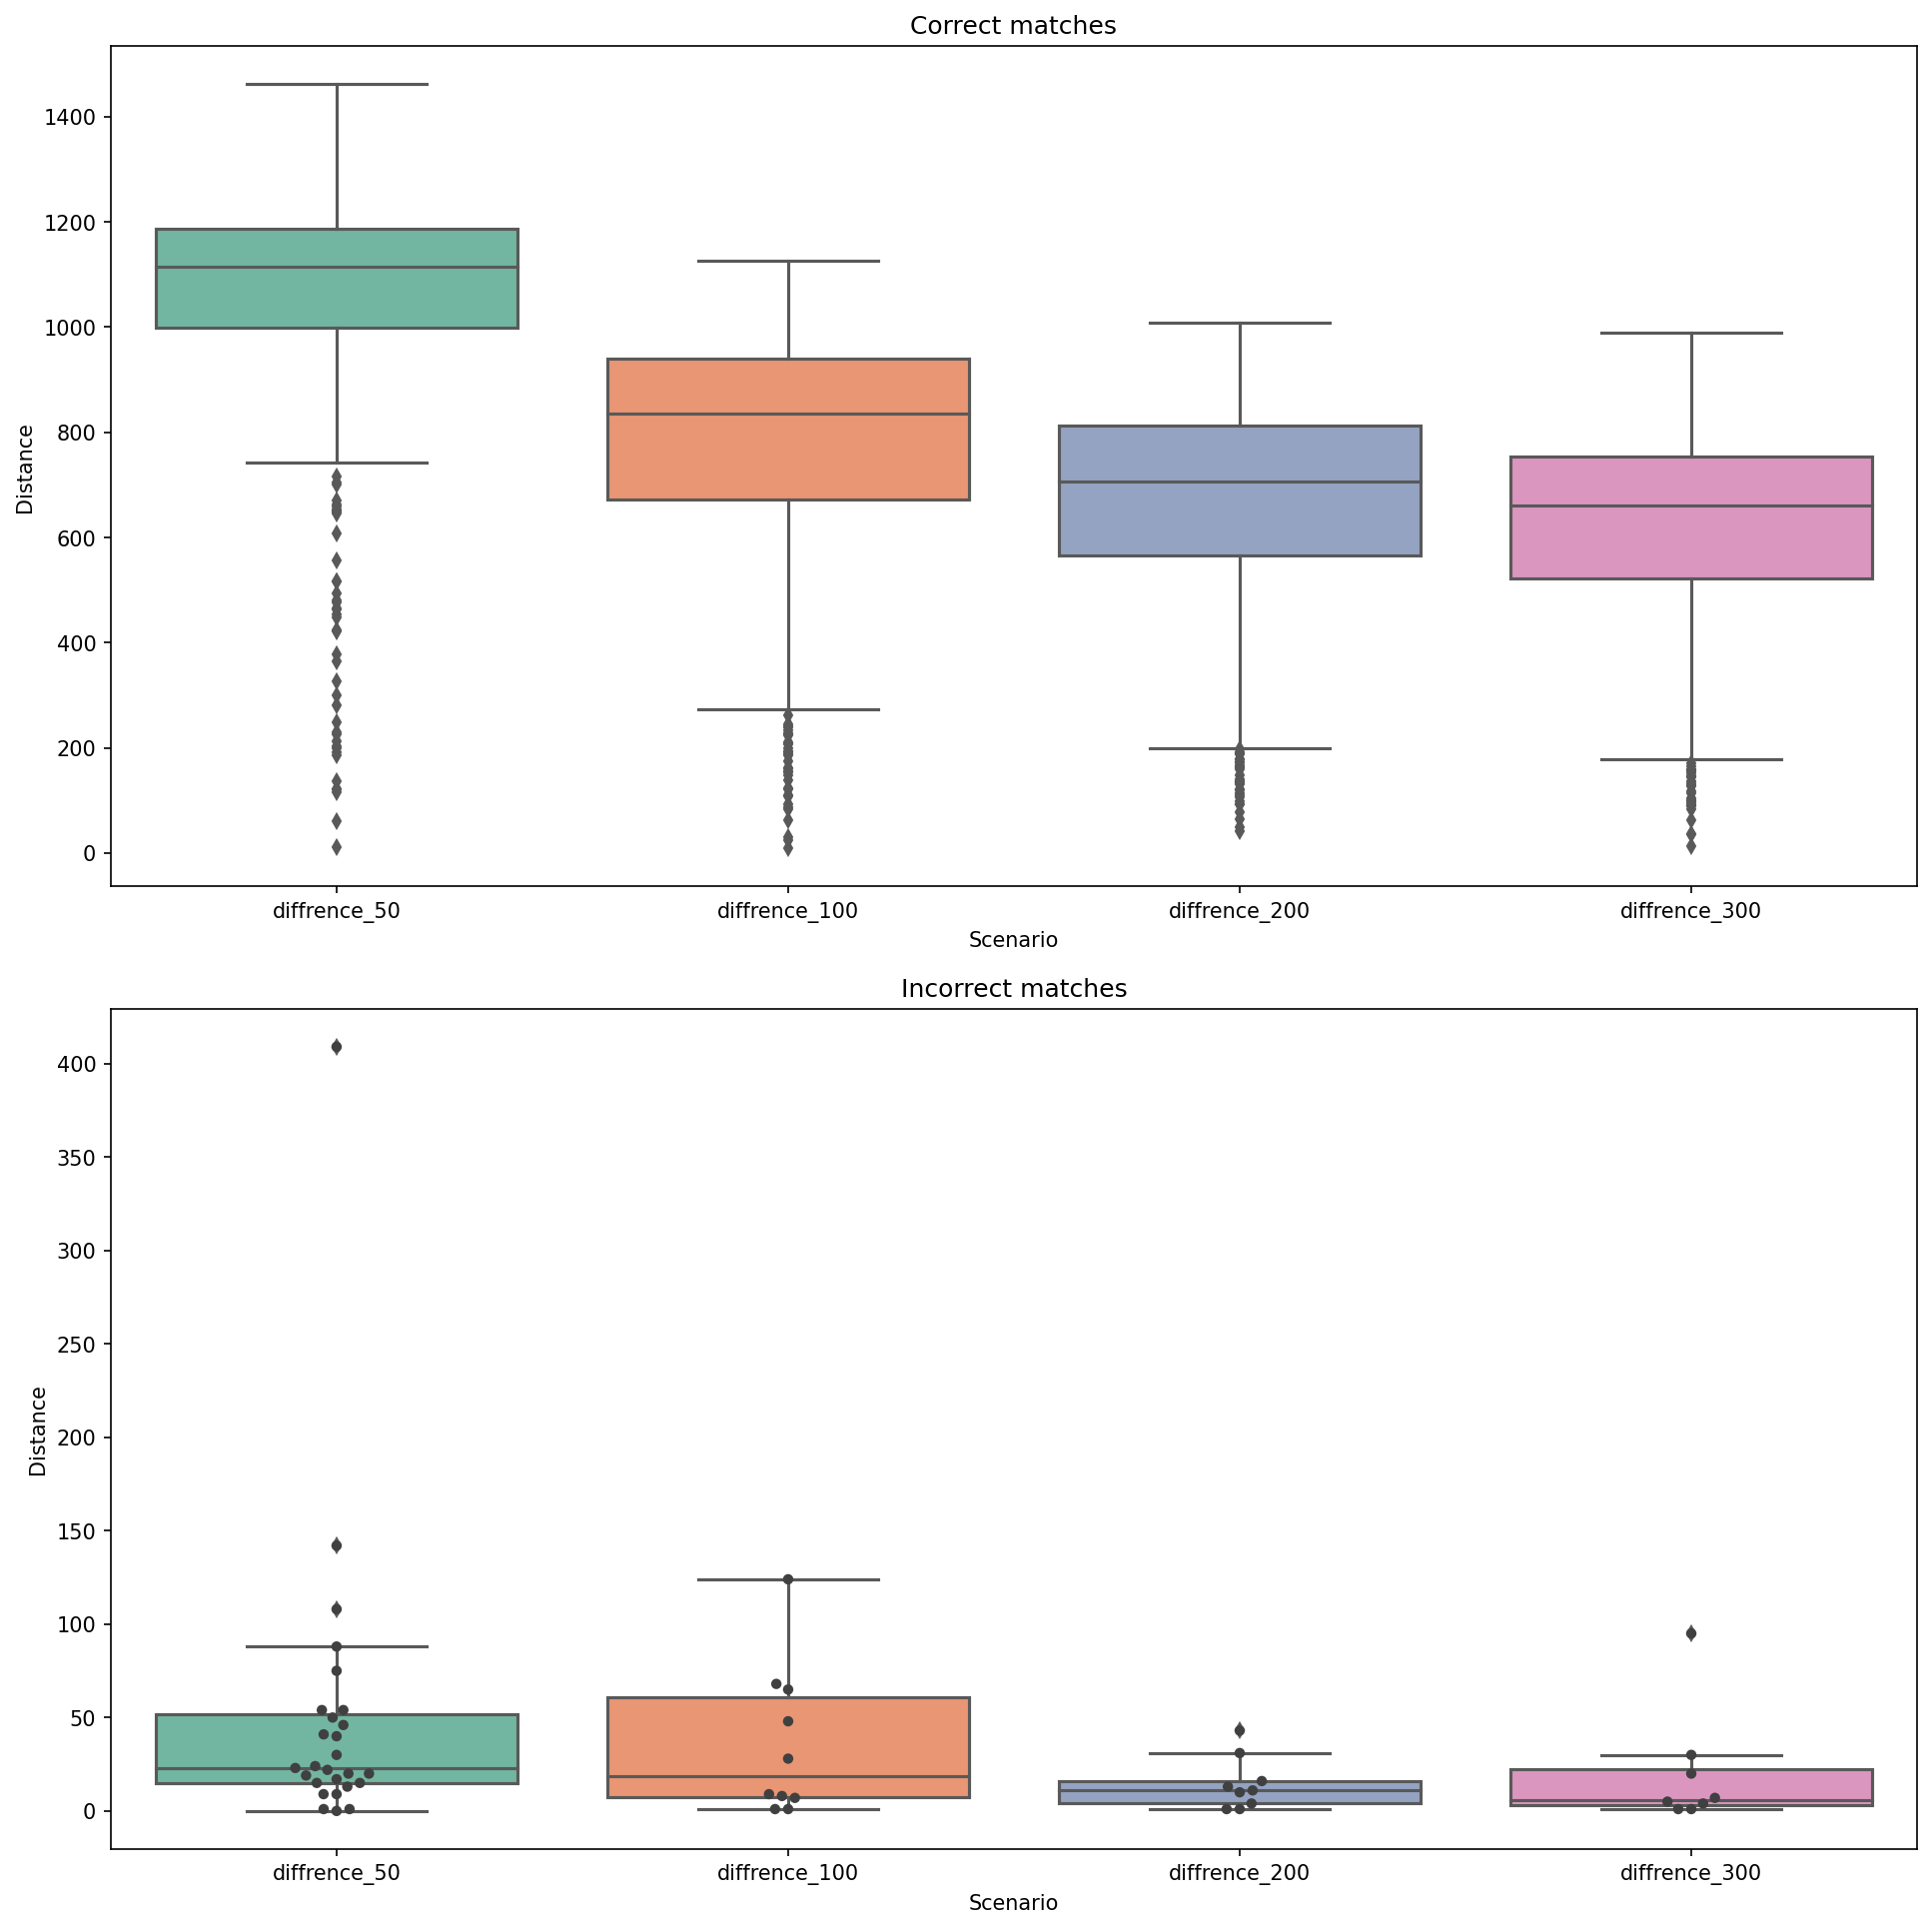
\includegraphics[width=1.0\columnwidth]{images/bxplt_difference_keypoints.png}
    \centering
    \caption{Difference in distance between the first and second matching result}
    \label{fig:bxplt_difference_keypoints}
\end{figure}

Earlier the chosen amount of keypoints/features was made on the matching score. In addition, the time to match one image is also a decisive factor. Table \ref{tab:keypoint_timing} illustrates the average time to match an image to the database. The matcher with 200 keypoints/features needs a double amount of time compared to the matcher with only 100 keypoints/features. Because of the realtime requirements, the choice for 100 keypoints is obvious.

% Time evaluation
\renewcommand{\arraystretch}{1.2}
\begin{table}[htbp]
    \caption{Keypoint/feature variation compute time}
    \centering
    \begin{center}
        \begin{tabular}{ |c|c|  }
         \hline
         No. of keypoints& Compute time (ms)\\
         \hline \hline
         50  & 60 \\
         \hline
         100 & 107 \\
         \hline
         200 & 238 \\
         \hline
         300 & 353 \\
         \hline
        \end{tabular}
    \end{center}
    \label{tab:keypoint_timing}
\end{table}

% importance of scaling
\subsection{Feature vector matching}
\label{subsec:Feature vector matching}

Our approach for feature vector matching relies on feature
extracting with a pre-trained model. The chosen model is
VGG16 with weights from imagenet. Such a model provides
interesting feature generation which is convenient for applying distance measurements \cite{feature_extraction}.

Figure \ref{fig:vgg16} illustrates all layers. The red square around the fully connected layer represents the prediction layer. This (dense) layer was cut off to obtain the feature vectors.

\begin{figure}[htbp]
    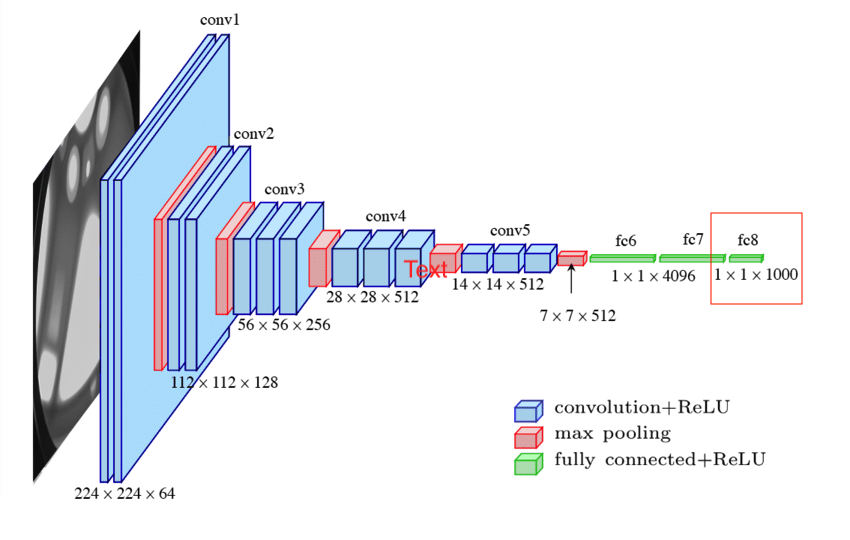
\includegraphics[width=1.0\columnwidth]{images/vgg16.png}
    \centering
    \caption{VGG16 layer visualization \cite{vgg16_image}}
    \label{fig:vgg16}
\end{figure}

Various distance metrics are applicable to obtain a distance result between the feature vectors. The following common metrics were evaluated: euclidean, cityblock, Minkowski, Chebyshev, and cosine. Table \ref{tab:fvector_score} shows the matching results on the same evaluation dataset in \ref{subsec:Keypoint matching}. Euclidean seems to have the highest positive ratio. The cityblock and cosine metrics also have acceptable scores. Only Chebyshev scores substandard.

%https://pdodds.w3.uvm.edu/research/papers/others/everything/cha2007a.pdf

\renewcommand{\arraystretch}{1.2}
\begin{table}[htbp]
    \caption{Distance metric variation correctness results}
    \centering
    \begin{center}
        \begin{tabular}{ |c|c|c|c|  }
         \hline
         Metric& Positive matches &Negative matches&Mean score (\%)\\
         \hline \hline
         euclidean & 363 & 74 & 83.07\\
         \hline
         cityblock & 358 & 79 & 81.92\\
         \hline
         chebyshev & 315 & 122 & 72.08\\
         \hline
         cosine & 360 & 77 & 82.38\\
         \hline
        \end{tabular}
    \end{center}
    \label{tab:fvector_score}
\end{table}

Each distance metric results in another range of distance values. (Table \ref{tab:fvector_distance_mean}) Comparing the correct matches distribution with the incorrect matches, an overlapping region is established for each distance metric.

\renewcommand{\arraystretch}{1.2}
\begin{table}[htbp]
    \caption{Distance distribution average values}
    \centering
    \begin{center}
        \begin{tabular}{ |c|c|c|c|  }
        %  \hline
        %  \multicolumn{4}{|c|}{Keypoint/feature variation correctness results.} \\
         \hline 
         Metric& Mean & Mean match & Mean no match\\
         \hline \hline
         euclidean  & 49.70 & 302.66 & 1413.36\\
         \hline
         cityblock & 1420.49 & 1371.98 & 1640.33\\
         \hline
         chebyshev & 5.22 & 5.16 & 5.38\\
         \hline
         cosine & 0.16 & 0.14 & 0.24\\
         \hline
         \end{tabular}
    \end{center}
    \label{tab:fvector_distance_mean}
\end{table}

Despite this property, differences between the first and second matches are still useful. The mean values for the differences between the first and second matches are shown in table \ref{tab:fvector_difference_mean}.

\renewcommand{\arraystretch}{1.2}
\begin{table}[htbp]
    \caption{Difference in distance distribution average values}
    \centering
    \begin{center}
        \begin{tabular}{ |c|c|c| }
        %  \hline
        %  \multicolumn{4}{|c|}{Keypoint/feature variation correctness results.} \\
         \hline
         Metric& Mean match & Mean no match\\
         \hline \hline
         euclidean  & 11.64 & 1.78\\
         \hline
         cityblock & 356.85 & 54.80\\
         \hline
         chebyshev & 1.02 & 0.22\\
         \hline
         cosine & 0.08 & 0.02 \\
         \hline
        \end{tabular}
    \end{center}
    \label{tab:fvector_difference_mean}
\end{table}

% \begin{figure}[htbp]
%     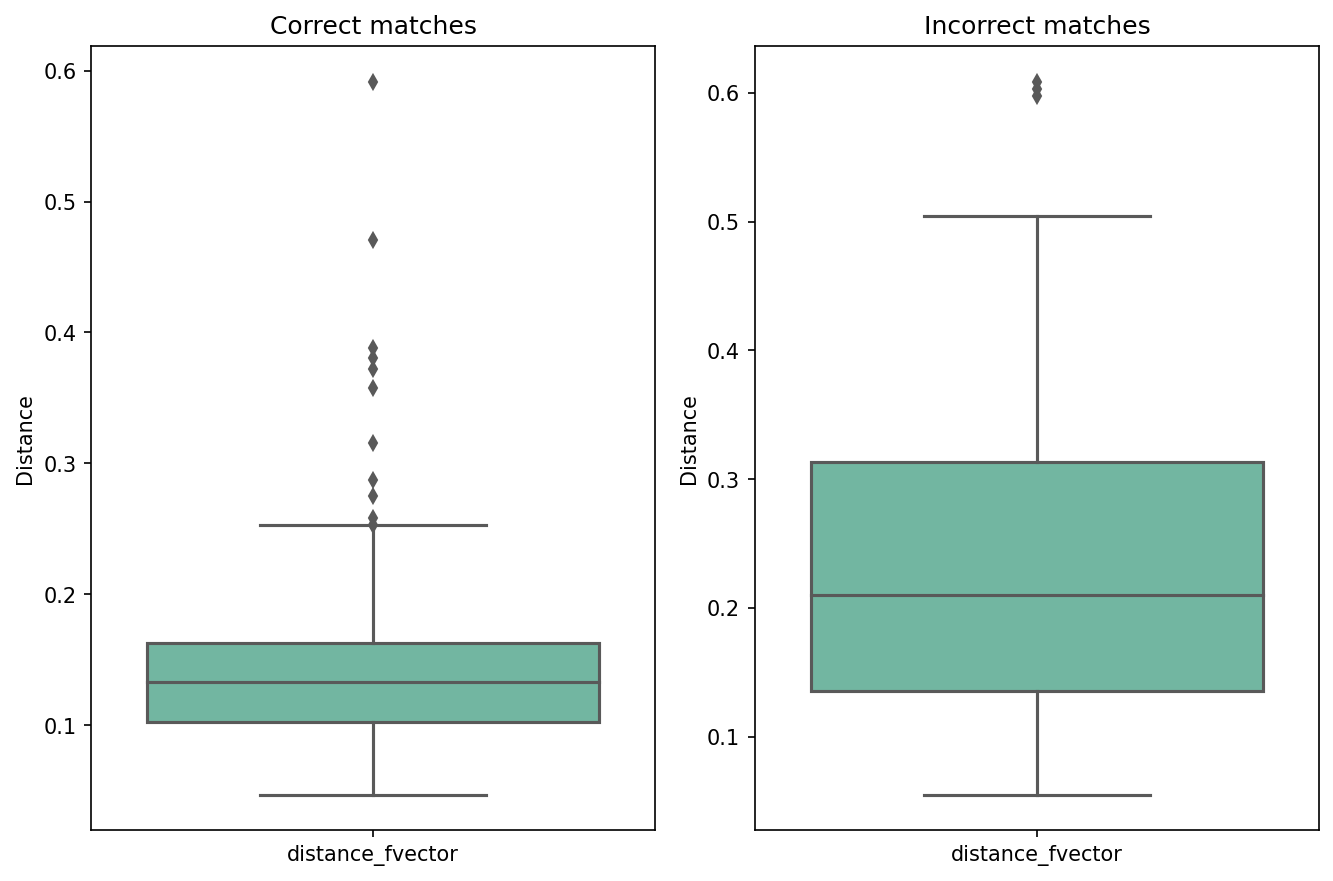
\includegraphics[width=0.8\columnwidth]{images/bxplt_distance_fvectors.png}
%     \centering
%     \caption{Distance distribution, left: correct matches | right: incorrect matches}
%     \label{fig:bxplt_distances_fvector}
% \end{figure}

% \begin{figure}[htbp]
%     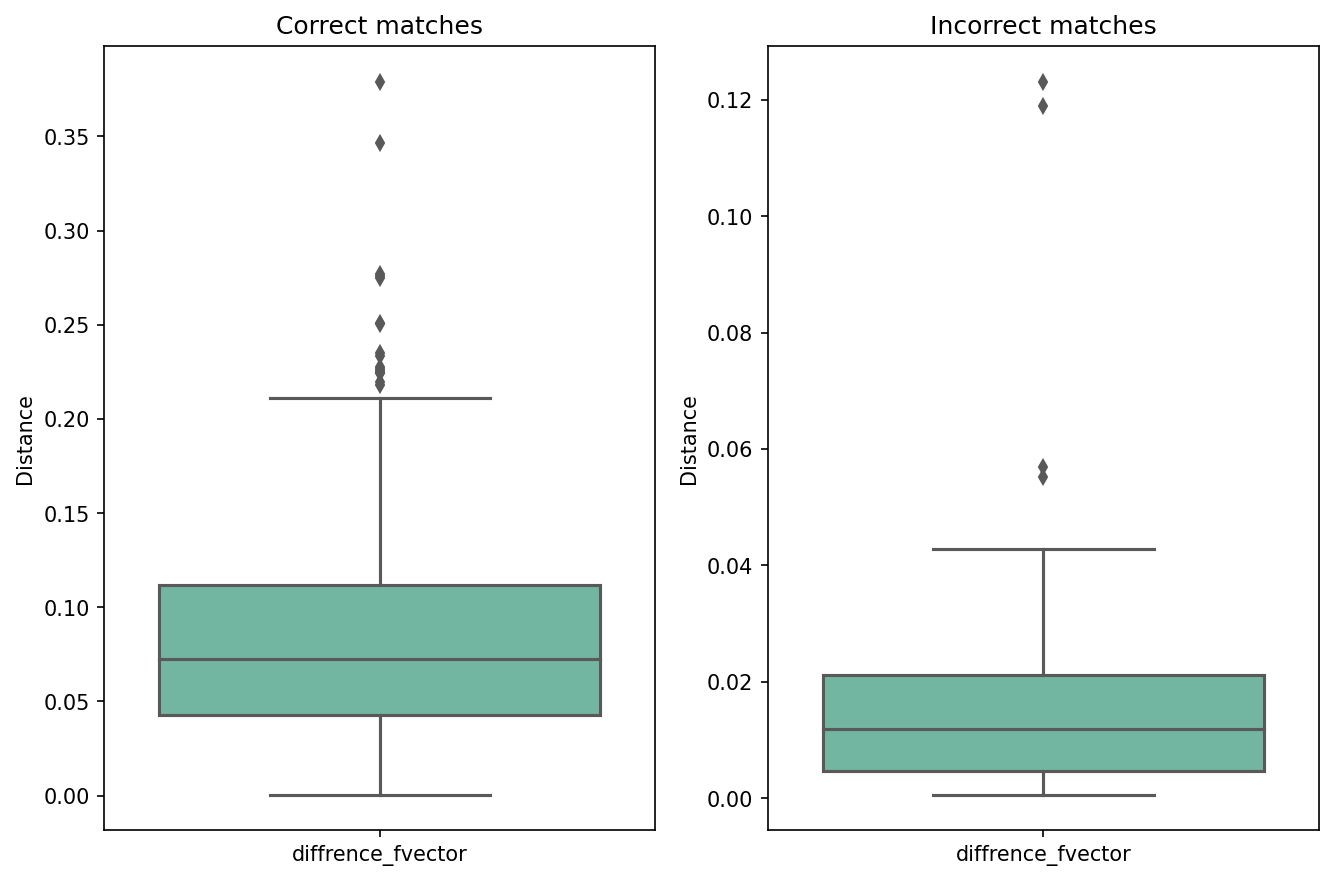
\includegraphics[width=0.8\columnwidth]{images/bxplt_difference_fvectors.png}
%     \centering
%     \caption{Difference between first and second matching result, left: correct matches | right: incorrect matches}
%     \label{fig:bxplt_diffrences_fvector}
% \end{figure}


Next to these distance and matching scores, time should also be taken into account when choosing a suitable distance metric. Table \ref{tab:fvector_timing} illustrates the average time to match an image upon the database. The matcher using the cityblock metric seems to have the fastest execution, followed by euclidean and cosine. The chebyshev version scores substandard again.

Based on the collected results euclidean and cityblock are the better choices. Both distance metrics are used to demonstrate the effects on the videos.

% Time evaluation
\renewcommand{\arraystretch}{1.2}
\begin{table}[htbp]
    \caption{Compute time distance metric dependent}
    \centering
    \begin{center}
        \begin{tabular}{ |c|c|  }
         \hline
         Distance metric& Compute time (ms)\\
         \hline \hline
         euclidean & 69.60\\
         \hline
         cityblock & 54.87\\
         \hline
         chebyshev & 221.30\\
         \hline
         cosine & 77.15\\
         \hline
        \end{tabular}
    \end{center}
    \label{tab:fvector_timing}
\end{table}

% distance pictures


\subsection{Matching evaluation}
\label{subsec:Matching evaluation}

All collected metrics for both matching approaches result in three final matchers which can be used in the realtime application: the keypoint-based matcher with 100 keypoints/features, the feature vector-based matching with euclidean distance metric, and the feature vector-based matching with cityblock distance metric.

The feature vector-based matchers have a faster compute time than the keypoint-based matcher while the keypoint-based matcher is more reliable in terms of correct matching. Because of this reason next to the implementations where only one kind of matcher is used, we also added a combination of a feature vector and a keypoint-based matcher.

This implementation takes advantage of the speed of the feature vector-based matcher. The matcher returns the first 50 images that may be a match. Next, the keypoint-based matcher only uses the 50 images which were returned by the feature vector-based matcher. The matching time for the keypoint-matcher is strongly reduced because only 50 images are considered instead of the whole database.

In general, one can conclude that the matching works well. It scores high when evaluating the dataset. In practice, as quoted before, blurry images and variant intensity caused by video usage still have an influence that cannot be ignored.